\documentclass[12pt,a4paper]{article}
\usepackage{amsfonts}
\usepackage{amsmath}
\usepackage{amsthm}
\usepackage[utf8]{inputenc}
\usepackage{hyperref}
\usepackage{booktabs}
\usepackage{graphicx}
%\usepackage{subcaption}

\graphicspath{ {fig/} }

\title{Lab 4}
\author{Santiago Bernal \\ Rodrigo Arias}

\begin{document}
\maketitle

\section*{Exercise 1}
%
% 1. Download from racó a python file named `exercise1_svm.py` in which you have
% to analyze three simple data sets.
%
In the file \texttt{ex1.py} three generators are used to provide 3 different 
random datasets.
%
% 2. For each data set you have a corresponding python function. In this
% function, you will call a SVM algorithm with three kernel functions. You will
% plot the hyperplane that separate the data set and its support vectors.
%
The SVM algorithm is applied to the train set of each dataset, and is plotted in 
the figures~\ref{fig:ex1gen1}, \ref{fig:ex1gen2} and~\ref{fig:ex1gen3}.
%
% 3. Make a prediction for the test data set with the SVM classifier and, in the
% console, write the number of instances correctly predicted and the total number
% of instances to predict. You can use sklearn library and the SVM algorithm
% included on it inside your python function.
%
The train data is shown with circle markers, while the test data uses crosses.  
The SVM decision regions are also filled with color, in order to visually see 
the behavior of the classifier.
%
% 4. In the report, for each one of the data sets, plot the different kernel
% functions analyzed and justify which is the best option for each one of them,
% taking into account that each data set has a different linear distribution.
%

We see that the datasets 1 and 3 are linearly separable, so a linear function 
should be used. The Gaussian kernel is used in the latter, but is behaving 
similarly to a linear kernel, so the classification is correct. The dataset 2, 
in contrast, is clearly not linearly separable, so a linear function should not 
be used. In the figure~\ref{fig:ex1gen2a} a Gaussian kernel was used, to see the 
difference. We see a better classification as expected.

The figure~\ref{fig:ex1gen2} shows a correct classification of 100\%, even if 
the classifier is not accurate. That can be explained because the test set 
provided with the generator, is only choosing elements that are placed in the 
outermost groups.
%
\begin{figure}[h]
	\centering
	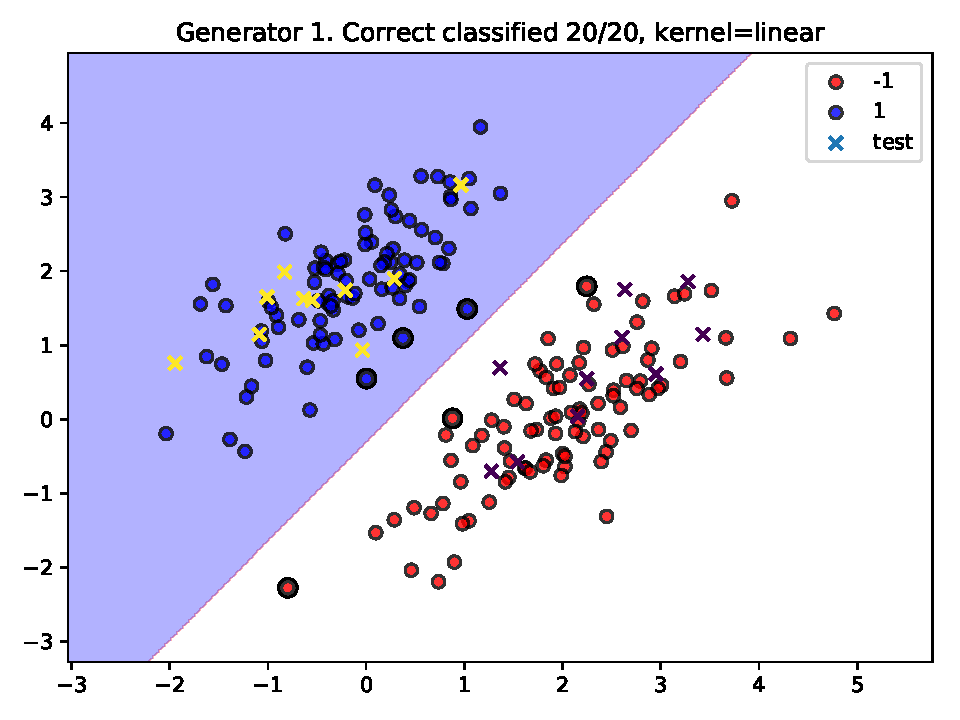
\includegraphics[width=0.7\textwidth]{ex1/1.pdf}
	\caption{Dataset of the generator 1}
	\label{fig:ex1gen1}
\end{figure}
\begin{figure}[h]
	\centering
	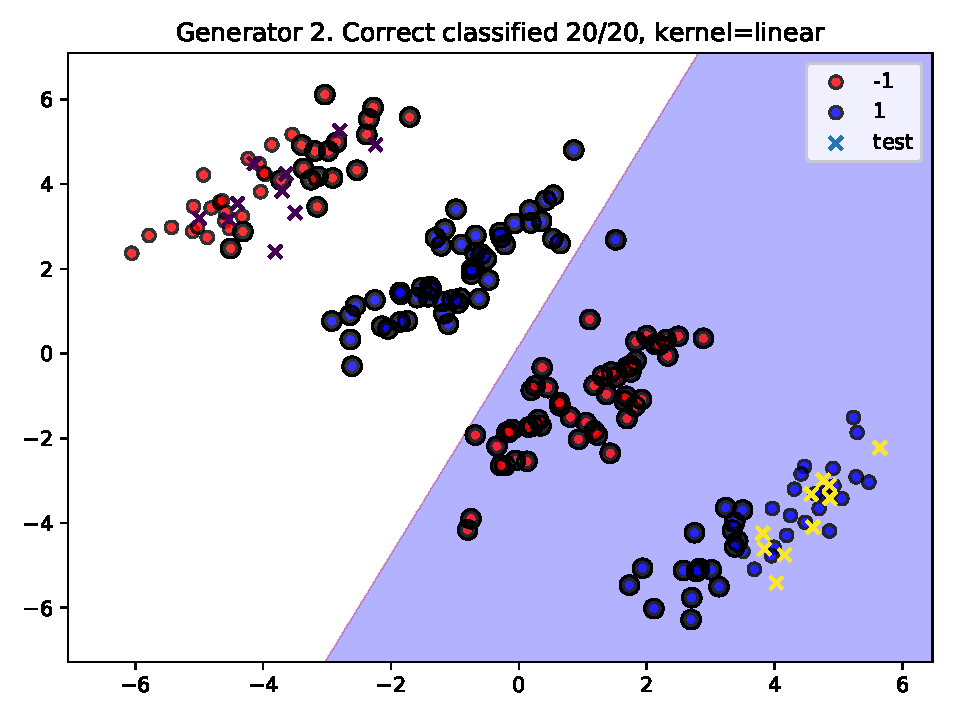
\includegraphics[width=0.7\textwidth]{ex1/2.pdf}
	\caption{Dataset of the generator 2}
	\label{fig:ex1gen2}
\end{figure}
\begin{figure}[h]
	\centering
	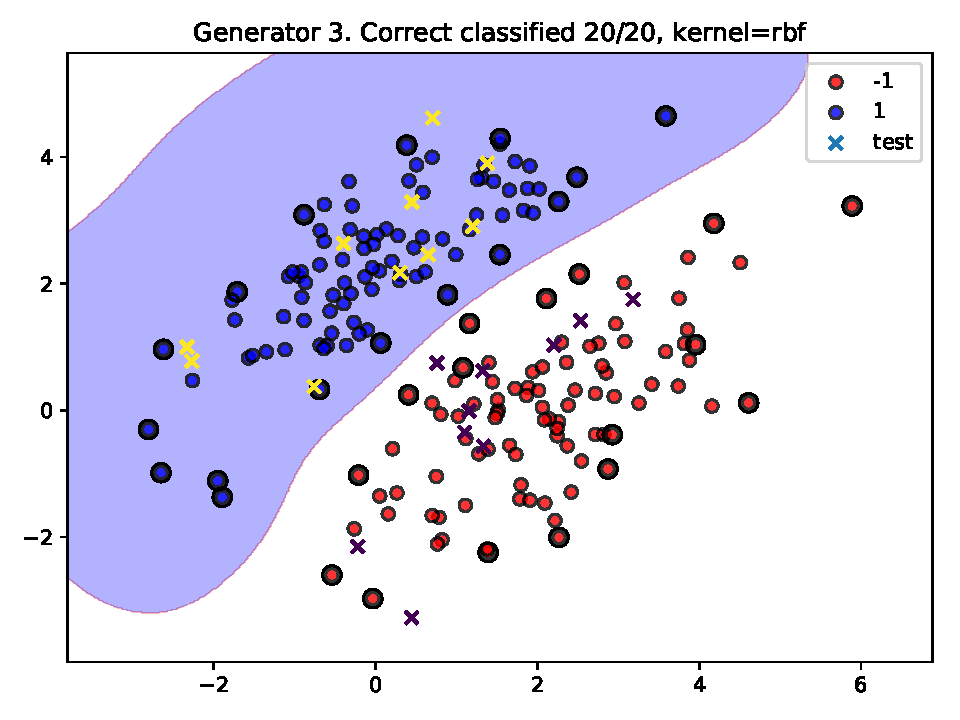
\includegraphics[width=0.7\textwidth]{ex1/3.pdf}
	\caption{Dataset of the generator 3}
	\label{fig:ex1gen3}
\end{figure}
\begin{figure}[h]
	\centering
	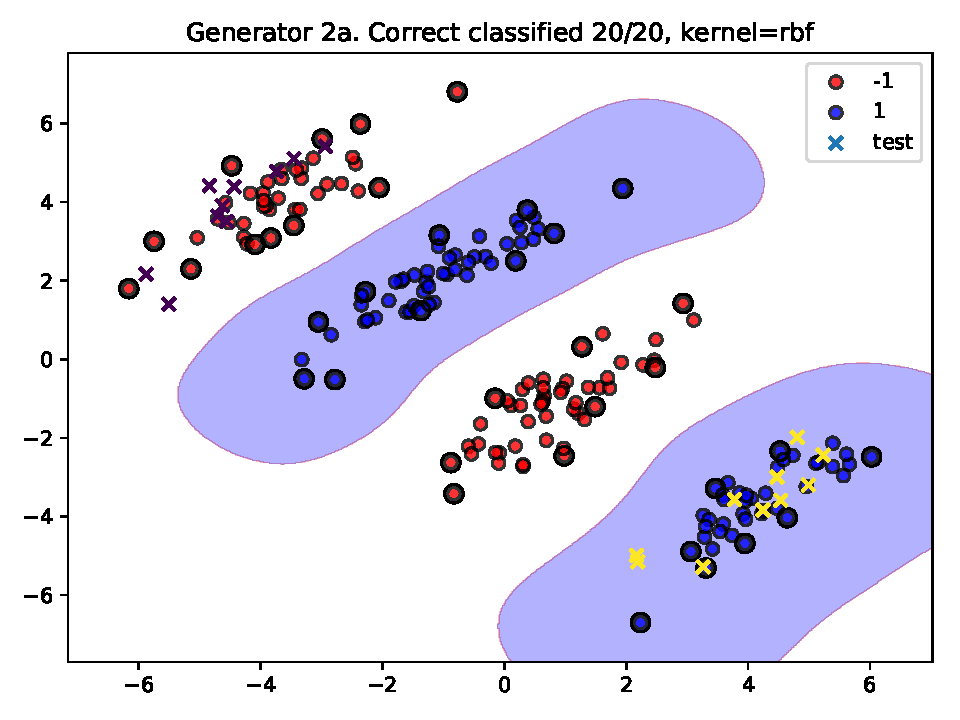
\includegraphics[width=0.7\textwidth]{ex1/2a.pdf}
	\caption{Dataset of the generator 2 using a Gaussian kernel}
	\label{fig:ex1gen2a}
\end{figure}
%

\end{document}
